% Wikshi Protocol — Whitepaper
% Compiled with pdfLaTeX
\documentclass[11pt,a4paper]{article}

% ── Geometry ──────────────────────────────────────────────────────────
\usepackage[
  top=2.8cm,
  bottom=2.5cm,
  left=2.5cm,
  right=2.5cm,
  headheight=14pt
]{geometry}

% ── Colors ────────────────────────────────────────────────────────────
\usepackage[dvipsnames,svgnames,x11names,table]{xcolor}

\definecolor{PrimaryDark}{HTML}{0D1B2A}
\definecolor{PrimaryMid}{HTML}{1B3A4B}
\definecolor{PrimaryAccent}{HTML}{00D4AA}
\definecolor{PrimaryLight}{HTML}{E0F7FA}
\definecolor{AccentGold}{HTML}{F5A623}
\definecolor{AccentBlue}{HTML}{2196F3}
\definecolor{TextPrimary}{HTML}{1A1A2E}
\definecolor{TextSecondary}{HTML}{4A5568}
\definecolor{DangerRed}{HTML}{FF6B6B}
\definecolor{BoxBg}{HTML}{F8FFFE}
\definecolor{SpecBg}{HTML}{0F2030}

% ── Typography ────────────────────────────────────────────────────────
\usepackage[T1]{fontenc}
\usepackage{lmodern}
\usepackage{microtype}
\usepackage{setspace}
\setstretch{1.15}
\setlength{\parskip}{0.4em}
\setlength{\parindent}{0pt}

% ── Math ──────────────────────────────────────────────────────────────
\usepackage{amsmath,amssymb,amsfonts}

% ── Graphics & Figures ────────────────────────────────────────────────
\usepackage{graphicx}
\usepackage{float}
\usepackage[font={small,color=TextSecondary},labelfont={bf,color=PrimaryMid}]{caption}

% ── Tables ────────────────────────────────────────────────────────────
\usepackage{booktabs}
\usepackage{tabularx}
\usepackage{array}
\newcolumntype{L}[1]{>{\raggedright\arraybackslash}p{#1}}
\newcolumntype{C}[1]{>{\centering\arraybackslash}p{#1}}

% ── TikZ ──────────────────────────────────────────────────────────────
\usepackage{tikz}
\usetikzlibrary{shapes.geometric,calc,positioning,backgrounds,patterns,shadows,fadings,decorations.pathmorphing,arrows.meta}

% ── Tagging stubs (tcolorbox 6.9.0 expects LaTeX 2025 tagging API) ────
\makeatletter
\@ifundefined{NewTaggingSocket}{%
  \newcommand{\NewTaggingSocket}[2]{\NewSocket{tagsupport/#1}{#2}}%
  \newcommand{\NewTaggingSocketPlug}[3]{}%
  \newcommand{\AssignTaggingSocketPlug}[2]{}%
}{}
\@ifundefined{NewStructureName}{%
  \newcommand{\NewStructureName}[1]{}%
  \newcommand{\AssignStructureRole}[2]{}%
  \newcommand{\UseStructureName}[1]{}%
}{}
\@ifundefined{tagstructbegin}{%
  \newcommand{\tagstructbegin}[1]{}%
  \newcommand{\tagstructend}{}%
}{}
\@ifundefined{tagpdfparaOff}{%
  \newcommand{\tagpdfparaOff}{}%
}{}
\makeatother

% ── Styled Boxes ──────────────────────────────────────────────────────
\usepackage[skins,breakable]{tcolorbox}

\newtcolorbox{keyinsight}{
  enhanced,
  breakable,
  colback=BoxBg,
  colframe=PrimaryAccent,
  leftrule=3pt,
  rightrule=0pt,
  toprule=0pt,
  bottomrule=0pt,
  arc=2mm,
  left=10pt,
  right=10pt,
  top=8pt,
  bottom=8pt,
  fontupper=\small,
  before skip=10pt,
  after skip=10pt
}

\newtcolorbox{definitionbox}[1][]{
  enhanced,
  breakable,
  colback=white,
  colframe=AccentBlue,
  leftrule=3pt,
  rightrule=0.5pt,
  toprule=0.5pt,
  bottomrule=0.5pt,
  arc=2mm,
  left=10pt,
  right=10pt,
  top=8pt,
  bottom=8pt,
  fontupper=\small,
  title={\sffamily\bfseries\color{AccentBlue}#1},
  coltitle=AccentBlue,
  attach boxed title to top left={yshift=-2mm,xshift=5mm},
  boxed title style={colback=white,colframe=white,sharp corners},
  before skip=10pt,
  after skip=10pt
}

\newtcolorbox{warningbox}{
  enhanced,
  breakable,
  colback=AccentGold!5,
  colframe=AccentGold,
  leftrule=3pt,
  rightrule=0pt,
  toprule=0pt,
  bottomrule=0pt,
  arc=2mm,
  left=10pt,
  right=10pt,
  top=8pt,
  bottom=8pt,
  fontupper=\small,
  before skip=10pt,
  after skip=10pt
}

% ── Section Styling ───────────────────────────────────────────────────
\usepackage{titlesec}

\titleformat{\section}
  {\Large\bfseries\sffamily\color{PrimaryMid}}
  {\colorbox{PrimaryAccent}{\makebox[2em][c]{\color{white}\thesection}}}
  {0.8em}
  {}
  [\vspace{-0.6em}{\color{PrimaryAccent}\rule{\textwidth}{1.5pt}}]

\titleformat{\subsection}
  {\large\bfseries\sffamily\color{PrimaryMid}}
  {\color{PrimaryAccent}\thesubsection}
  {0.6em}
  {}

\titleformat{\subsubsection}
  {\normalsize\bfseries\sffamily\color{TextSecondary}}
  {\color{TextSecondary}\thesubsubsection}
  {0.5em}
  {}

\titlespacing*{\section}{0pt}{1.5em}{0.8em}
\titlespacing*{\subsection}{0pt}{1.2em}{0.5em}
\titlespacing*{\subsubsection}{0pt}{0.8em}{0.3em}

% ── Headers & Footers ────────────────────────────────────────────────
\usepackage{fancyhdr}
\pagestyle{fancy}
\fancyhf{}
\fancyhead[L]{\small\color{TextSecondary}\sffamily Wikshi Protocol}
\fancyhead[R]{\small\color{TextSecondary}\sffamily\nouppercase{\leftmark}}
\fancyfoot[C]{{\color{PrimaryAccent}\rule{4cm}{0.8pt}}\\[3pt]\small\color{TextSecondary}\thepage}
\renewcommand{\headrulewidth}{0pt}

% ── Lists ─────────────────────────────────────────────────────────────
\usepackage{enumitem}
\setlist[itemize]{
  label={\color{PrimaryAccent}$\blacktriangleright$},
  leftmargin=1.5em,
  itemsep=2pt,
  parsep=0pt
}
\setlist[enumerate]{
  label={\color{PrimaryAccent}\bfseries\arabic*.},
  leftmargin=1.8em,
  itemsep=2pt,
  parsep=0pt
}

% ── Links ─────────────────────────────────────────────────────────────
\usepackage[
  colorlinks=true,
  linkcolor=PrimaryMid,
  citecolor=PrimaryAccent,
  urlcolor=AccentBlue,
  bookmarks=true,
  bookmarksnumbered=true
]{hyperref}

% ── Custom Commands ───────────────────────────────────────────────────
\sloppy
\newcommand{\protocol}{\textsc{Wikshi}}
\newcommand{\creditcoin}{\textsc{Creditcoin}}

% ══════════════════════════════════════════════════════════════════════
\begin{document}

% ── TITLE PAGE ────────────────────────────────────────────────────────
\begin{titlepage}
\begin{tikzpicture}[remember picture, overlay]
  % Dark background
  \fill[PrimaryDark] (current page.south west) rectangle (current page.north east);

  % --- Hexagonal network pattern (top region) ---
  \begin{scope}[opacity=0.18]
    \foreach \x/\y/\s in {
      1.5/25.5/1.4, 4.5/26.0/1.0, 7.0/25.0/1.6, 10.0/26.5/0.9,
      13.0/25.5/1.3, 16.0/26.0/1.1, 19.0/25.0/1.5,
      2.5/23.0/1.1, 5.5/23.5/1.5, 8.5/22.5/0.8, 11.5/23.0/1.2,
      14.5/23.5/1.0, 17.5/22.5/1.4, 20.0/23.0/0.9
    }{
      \node[regular polygon, regular polygon sides=6, minimum size=\s cm,
            draw=PrimaryAccent, line width=1.8pt, rotate=30] at (\x,\y) {};
    }
  \end{scope}

  % --- Hexagonal network pattern (bottom region) ---
  \begin{scope}[opacity=0.12]
    \foreach \x/\y/\s in {
      1.0/4.5/1.2, 4.0/3.5/0.9, 7.0/4.0/1.5, 10.0/3.0/1.0,
      13.0/4.5/1.3, 16.0/3.5/0.8, 19.0/4.0/1.4,
      2.5/6.5/0.8, 5.5/7.0/1.1, 8.5/6.0/1.3, 11.5/7.0/0.9,
      14.5/6.5/1.2, 17.5/7.0/1.0, 20.0/6.0/0.7
    }{
      \node[regular polygon, regular polygon sides=6, minimum size=\s cm,
            draw=PrimaryAccent, line width=1.5pt, rotate=30] at (\x,\y) {};
    }
  \end{scope}

  % --- Large faded hexagons (background texture) ---
  \begin{scope}[opacity=0.06]
    \foreach \x/\y/\s in {
      3/15/3.5, 17/17/4.0, 10/10/3.0, 1/20/2.5, 19/12/3.2
    }{
      \node[regular polygon, regular polygon sides=6, minimum size=\s cm,
            fill=PrimaryAccent, rotate=30] at (\x,\y) {};
    }
  \end{scope}

  % --- Accent bar (centered vertically between bottom info and tagline) ---
  \fill[PrimaryAccent, opacity=0.9]
    ([yshift=-0.4cm]current page.center -| current page.west)
    rectangle
    ([yshift=-0.2cm]current page.center -| current page.east);

  % --- Title block (centered on page) ---
  \node[anchor=center, text=white, font=\fontsize{44}{50}\selectfont\sffamily\bfseries]
    at ([yshift=4.5cm]current page.center) {Wikshi Protocol};

  \node[anchor=center, text=PrimaryAccent, font=\fontsize{18}{22}\selectfont\sffamily]
    at ([yshift=2.8cm]current page.center) {Credit-Native Lending on Creditcoin};

  \node[anchor=center, text=white!80, font=\fontsize{12}{16}\selectfont\sffamily,
        text width=14cm, align=center]
    at ([yshift=1.2cm]current page.center) {%
      Where verified repayment history unlocks better borrowing terms};

  % --- Bottom info block ---
  \node[anchor=center, text=AccentGold, font=\fontsize{11}{13}\selectfont\sffamily]
    at ([yshift=-2.5cm]current page.center) {Version 1.0 \quad$\cdot$\quad March 2026};

  \node[anchor=center, text=white!60, font=\fontsize{11}{14}\selectfont\sffamily]
    at ([yshift=-3.7cm]current page.center) {Miny Labs};

  \node[anchor=center, text=white!35, font=\fontsize{9}{11}\selectfont\sffamily]
    at ([yshift=-5.0cm]current page.center) {akash@miny-labs.com};

\end{tikzpicture}
\end{titlepage}

% ── TABLE OF CONTENTS ─────────────────────────────────────────────────
\newpage
\tableofcontents
\thispagestyle{fancy}
\newpage

% ══════════════════════════════════════════════════════════════════════
% ABSTRACT
% ══════════════════════════════════════════════════════════════════════
\section*{Abstract}
\addcontentsline{toc}{section}{Abstract}

Decentralized lending protocols require all borrowers to post the same collateral regardless of creditworthiness---a first-time user and a wallet with years of clean repayment history face identical terms. Wikshi addresses this by building a credit-adjusted lending protocol on Creditcoin that reads verified payment history from multiple chains and translates it into individualized borrowing parameters. The protocol ingests credit events through three channels---cross-chain cryptographic proofs via Creditcoin's Universal Smart Contract (USC) infrastructure, native Creditcoin loan events, and an off-chain credit API---and computes an on-chain credit score that dynamically modifies each borrower's collateral requirements (up to 10\% reduction) and interest rate (up to 20\% discount). A progressive trust tier system gates these benefits behind sustained good behavior, while score decay and liquidation slashing ensure that credit standing reflects ongoing performance. Wikshi also implements a receivables pipeline that tokenizes real-world microfinance loans into fungible DeFi collateral through credit-adjusted discounted cash flow valuation. The architecture follows the Morpho Blue singleton pattern---one contract, infinite isolated markets, permissionless composition.

\vspace{1em}

% ══════════════════════════════════════════════════════════════════════
% 1. INTRODUCTION
% ══════════════════════════════════════════════════════════════════════
\section{Introduction}

\subsection{The Credit Gap in DeFi}

The global unsecured credit market exceeds \$5.3 trillion.\footnote{Market Research Future, ``Unsecured Business Loans Market Forecast to 2032.''} Cash-flow-based financing---where creditworthiness rather than collateral determines access to capital---represents another \$1.3 trillion.\footnote{Allied Market Research, ``Cash Flow Lending Market, 2032.''} Traditional finance allocates capital based on demonstrated ability to repay. DeFi does not.

Every major lending protocol---Aave, Compound, Spark---treats all borrowers identically. A first-time wallet and one with five years of perfect repayment history both post 150\% collateral for the same loan. This flat-rate approach made sense when on-chain identity was nonexistent, but it creates a structural inefficiency: capital is locked that does not need to be, and borrowers who have demonstrated creditworthiness receive no benefit from it.

The numbers are concrete. On Aave V3, borrowing \$10{,}000 USDC against ETH requires approximately \$15{,}000 in collateral at the standard 66.5\% loan-to-value ratio. A borrower who has repaid 50 loans without a single late payment posts the same amount as someone borrowing for the first time. The difference in risk between these two borrowers is real---the protocol simply cannot measure it.

Several protocols have attempted to bring credit into DeFi. Goldfinch~\cite{goldfinch} relies on human auditors to vet borrower pools---effective but slow and non-scalable. 3Jane~\cite{threejane} uses zkTLS to pull off-chain credit scores and issue fully unsecured credit lines---capital-efficient but eliminates the safety net of collateral entirely. Maple Finance~\cite{maple} serves institutional borrowers through off-chain due diligence and whitelisted pools---proven but inaccessible to the long tail of borrowers. None of these approaches combines the safety of collateralized lending with individualized credit adjustment.

\subsection{Creditcoin's Credit Infrastructure}

Creditcoin has built the largest on-chain credit dataset in decentralized finance. Through its partnerships with Aella (serving 2M+ borrowers across emerging markets) and integration with Gluwa's lending infrastructure, the network has recorded over 5 million real-world loan transactions representing more than \$80M in credit volume.\footnote{Creditcoin Foundation. The Central Bank of Nigeria signed an MOU to explore Creditcoin data for financial inclusion.}

Until now, none of this data has been usable inside a lending protocol. It sits on Creditcoin's Layer~1 as raw transaction history---valuable, verified, but inert.

Two pieces of infrastructure changed that. First, Creditcoin's Universal Smart Contract (USC) precompiles enable any smart contract on the Creditcoin EVM to verify transaction proofs from external chains.\footnote{USC v2 documentation: \url{https://docs.creditcoin.org/}} A loan payment made on Ethereum can be cryptographically verified on Creditcoin within 15 seconds using Merkle proofs and continuity proofs---no oracle, no bridge, no trust assumption beyond the source chain's consensus. Second, Creditcoin's native EVM layer exposes L1 loan events directly to smart contracts.

Wikshi is the first protocol to combine both.

\subsection{Protocol Summary}

Wikshi is a lending protocol where credit history determines borrowing terms. It occupies a specific position in the design space:

\begin{keyinsight}
\textbf{Collateralized lending with credit-based adjustment.} Wikshi preserves the safety properties of overcollateralized lending---every loan is backed by collateral---while progressively reducing requirements for borrowers who prove themselves through verified repayment history. This is distinct from unsecured credit (3Jane), human-audited trust networks (Goldfinch), or institutional whitelists (Maple).
\end{keyinsight}

The protocol has three primary components:

\begin{enumerate}
\item \textbf{Credit oracle.} Ingests payment events from USC cross-chain proofs, Creditcoin native events, and an off-chain API. Computes a score between 0 and 1000. Resolves a progressive trust tier that gates access to credit benefits.
\item \textbf{Core lending.} A singleton contract managing isolated markets with credit-adjusted parameters. Higher credit scores reduce collateral requirements (up to +10\% LLTV bonus) and interest rates (up to 20\% discount).
\item \textbf{RWA receivables pipeline.} Tokenizes real-world loan receivables into fungible ERC-20 collateral via credit-adjusted DCF valuation, bridging Creditcoin's existing credit infrastructure into composable DeFi capital.
\end{enumerate}

% ══════════════════════════════════════════════════════════════════════
% 2. PROTOCOL ARCHITECTURE
% ══════════════════════════════════════════════════════════════════════
\section{Protocol Architecture}

\subsection{System Overview}

Figure~\ref{fig:overview} shows the high-level architecture. The protocol is organized around four functional groups connected by well-defined interfaces.

\begin{figure}[H]
\centering
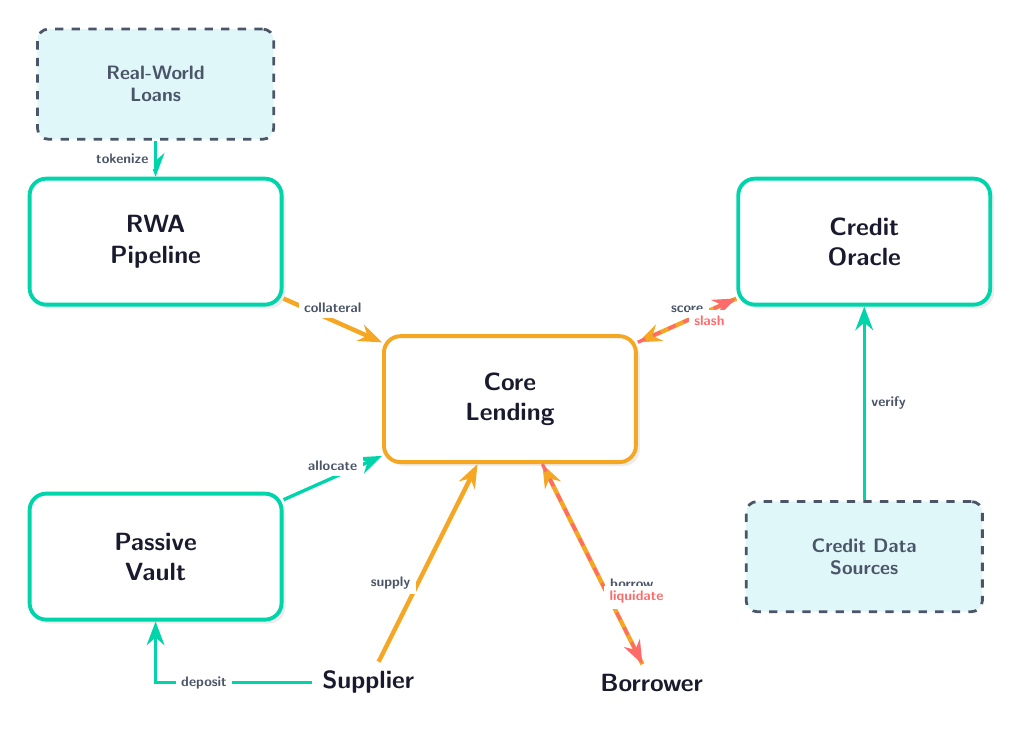
\begin{tikzpicture}[
  node distance=2.2cm and 2.8cm,
  box/.style={rectangle, rounded corners=6pt, draw=#1, fill=white,
              text=TextPrimary, line width=1.4pt, minimum width=3.2cm,
              minimum height=1.6cm, font=\sffamily\small\bfseries, align=center,
              drop shadow={shadow xshift=0.5mm, shadow yshift=-0.5mm, opacity=0.15}},
  box/.default=PrimaryAccent,
  extbox/.style={rectangle, rounded corners=4pt, draw=TextSecondary, dashed,
                 fill=PrimaryLight, text=TextSecondary, line width=1pt,
                 minimum width=3cm, minimum height=1.4cm,
                 font=\sffamily\scriptsize\bfseries, align=center},
  actor/.style={font=\sffamily\small\bfseries, text=TextPrimary},
  arr/.style={-{Stealth[length=3mm]}, line width=1.2pt, color=PrimaryAccent},
  garr/.style={-{Stealth[length=3mm]}, line width=1.6pt, color=AccentGold},
  rarr/.style={-{Stealth[length=3mm]}, line width=1.2pt, color=DangerRed, dashed},
  lbl/.style={font=\sffamily\tiny\bfseries, color=TextSecondary, fill=white, inner sep=2pt},
]
  % Core boxes
  \node[box=AccentGold] (lending) at (0,0) {Core\\Lending};
  \node[box] (oracle) at (4.5,2) {Credit\\Oracle};
  \node[box] (rwa) at (-4.5,2) {RWA\\Pipeline};
  \node[box] (vault) at (-4.5,-2) {Passive\\Vault};

  % External sources
  \node[extbox] (sources) at (4.5,-2) {Credit Data\\Sources};
  \node[extbox] (loans) at (-4.5,4) {Real-World\\Loans};

  % Actors
  \node[actor] (supplier) at (-1.8,-3.6) {Supplier};
  \node[actor] (borrower) at (1.8,-3.6) {Borrower};

  % Gold flows (core)
  \draw[garr] (borrower) -- node[lbl, right, pos=0.4] {borrow} (lending);
  \draw[garr] (supplier) -- node[lbl, left, pos=0.4] {supply} (lending);
  \draw[garr] (oracle) -- node[lbl, above, pos=0.5] {score} (lending);
  \draw[garr] (rwa) -- node[lbl, above, pos=0.5] {collateral} (lending);

  % Teal flows (data/periphery)
  \draw[arr] (sources) -- node[lbl, right, pos=0.5] {verify} (oracle);
  \draw[arr] (loans) -- node[lbl, left, pos=0.5] {tokenize} (rwa);
  \draw[arr] (vault) -- node[lbl, above, pos=0.5] {allocate} (lending);
  \draw[arr] (supplier) -| node[lbl, left, pos=0.25] {deposit} (vault);

  % Red flows (liquidation/slashing)
  \draw[rarr] (lending) -- node[lbl, right, pos=0.5] {\color{DangerRed}slash} (oracle);
  \draw[rarr] (lending) -- node[lbl, below right, pos=0.6] {\color{DangerRed}liquidate} (borrower);
\end{tikzpicture}
\caption{Wikshi system architecture. Gold connections represent core lending flows. Teal connections represent data and verification paths. Red dashed connections represent liquidation and slashing.}
\label{fig:overview}
\end{figure}

Credit data flows from external sources through the oracle into the lending engine, where it modifies per-borrower parameters. Real-world assets flow from loan originators through the tokenization pipeline into lending markets as collateral. Suppliers interact either directly with individual markets or through a passive vault that allocates across multiple markets.

\subsection{Isolated Market Design}

The lending engine follows the Morpho Blue singleton architectural pattern~\cite{morpho}: a single immutable contract manages an unbounded number of fully isolated markets. Each market is defined by five parameters---loan token, collateral token, price oracle, interest rate model, and base loan-to-value ratio. Markets are permissionless: anyone can create one by specifying valid parameters.

This contrasts with the shared-pool model used by Aave and Compound, where all collateral types share risk within a single lending pool. The singleton approach eliminates pool-level contagion---a default in one market cannot cascade to another---at the cost of liquidity fragmentation. This tradeoff is acceptable for the long-tail asset markets Wikshi targets: wrapped microfinance receivables, emerging market stablecoins, and CTC-denominated instruments.

Supply and borrow positions are tracked internally as \emph{shares} rather than absolute token amounts. When interest accrues, the total borrow amount increases but total shares remain constant---each share becomes worth more tokens. Virtual share offsets prevent the well-known first-depositor inflation attack.\footnote{The attack involves a small first deposit followed by a large direct transfer to manipulate the share price. Virtual offsets make this economically unviable.}

% ══════════════════════════════════════════════════════════════════════
% 3. CREDIT SYSTEM
% ══════════════════════════════════════════════════════════════════════
\section{Credit System}

The credit system is Wikshi's core differentiator. It transforms raw payment events into a borrower-specific score that modifies lending parameters in real time.

\subsection{Dual-Source Credit Oracle}

The oracle ingests credit events from three distinct channels that span the Creditcoin ecosystem:

\textbf{Cross-chain verification (USC).} Borrowers submit cryptographic proofs of loan payments made on external EVM chains. The Creditcoin USC infrastructure verifies Merkle and continuity proofs at the protocol level, then the oracle decodes the verified transaction to extract the payment event.\footnote{USC precompiles are deployed at fixed addresses on the Creditcoin EVM. The VerifierInterface accepts a chain key, block height, encoded transaction, Merkle proof, and continuity proof. See Creditcoin USC v2 documentation.} Recognized events include general payment confirmations and Gluwa Loan.sol lifecycle events: loan funding, repayment, late repayment, and expiration.

\textbf{Creditcoin native events.} The protocol directly processes loan events generated on Creditcoin's Layer~1---the same events created by the 5M+ transactions already on the network. These require no cross-chain proof; they are native to the execution environment.

\textbf{Credal operator.} An authorized off-chain operator can submit score updates directly. This channel is compatible with Creditcoin's Credal API infrastructure, which powers real-world lending for partners like Aella. The operator role is pluggable---any lender's risk model can be integrated without modifying the on-chain contracts.

\begin{figure}[H]
\centering
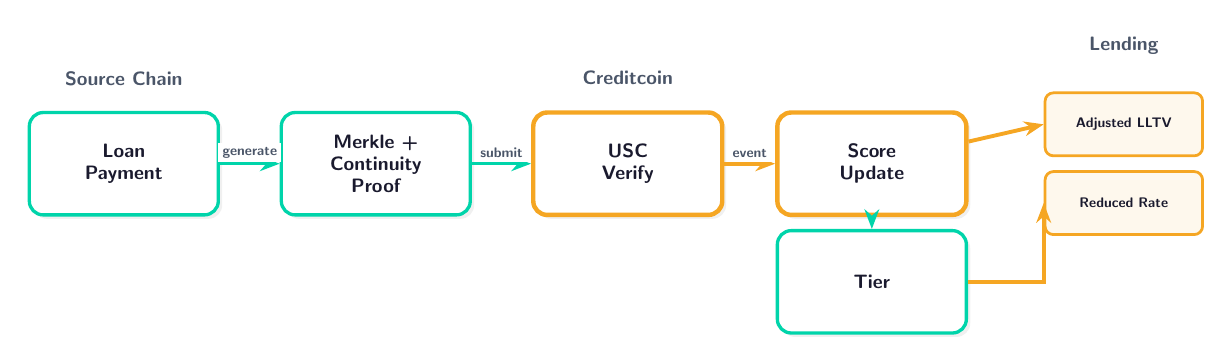
\begin{tikzpicture}[
  node distance=0.8cm,
  sbox/.style={rectangle, rounded corners=5pt, draw=PrimaryAccent, fill=white,
               text=TextPrimary, line width=1.2pt, minimum width=2.4cm, minimum height=1.3cm,
               font=\sffamily\scriptsize\bfseries, align=center,
               drop shadow={shadow xshift=0.5mm, shadow yshift=-0.5mm, opacity=0.12}},
  highlight/.style={sbox, draw=AccentGold, line width=1.6pt},
  result/.style={rectangle, rounded corners=3pt, draw=AccentGold, fill=AccentGold!8,
                 text=TextPrimary, line width=1pt, minimum width=2cm, minimum height=0.8cm,
                 font=\sffamily\tiny\bfseries, align=center},
  arr/.style={-{Stealth[length=2.5mm]}, line width=1.2pt, color=PrimaryAccent},
  garr/.style={-{Stealth[length=2.5mm]}, line width=1.4pt, color=AccentGold},
  lbl/.style={font=\sffamily\tiny\bfseries, color=TextSecondary, fill=white, inner sep=1.5pt},
  grplbl/.style={font=\sffamily\scriptsize\bfseries, color=TextSecondary},
]
  % Stage 1: Source Chain
  \node[sbox] (payment) at (-6.5,0) {Loan\\Payment};
  \node[grplbl, above=0.2cm of payment] {Source Chain};

  % Stage 2: Proof
  \node[sbox] (proof) at (-3.3,0) {Merkle +\\Continuity\\Proof};

  % Stage 3: USC Verification
  \node[highlight] (verify) at (-0.1,0) {USC\\Verify};
  \node[grplbl, above=0.2cm of verify] {Creditcoin};

  % Stage 4: Oracle
  \node[highlight] (score) at (3,0) {Score\\Update};
  \node[sbox] (tier) at (3,-1.5) {Tier};

  % Stage 5: Results
  \node[result] (lltv) at (6.2,0.5) {Adjusted LLTV};
  \node[result] (rate) at (6.2,-0.5) {Reduced Rate};
  \node[grplbl, above=0.35cm of lltv] {Lending};

  % Arrows
  \draw[arr] (payment) -- node[lbl, above] {generate} (proof);
  \draw[arr] (proof) -- node[lbl, above] {submit} (verify);
  \draw[garr] (verify) -- node[lbl, above] {event} (score);
  \draw[arr] (score) -- (tier);
  \draw[garr] (score) -- (lltv.west);
  \draw[garr] (tier) -| (rate.west);
\end{tikzpicture}
\caption{Credit verification pipeline. Payment events on source chains generate cryptographic proofs verified by Creditcoin's USC infrastructure, decoded into credit score and tier updates that adjust lending parameters.}
\label{fig:credit-verify}
\end{figure}

\subsection{Score Mechanics}

Credit scores range from 0 to 1000. A new borrower starts with no record; scores are initialized at 300 upon the first verified credit event.

The score increment depends on the verified payment amount:

\begin{equation}
\Delta s = \begin{cases}
  30 & \text{if payment} \geq \$1{,}000 \\
  20 & \text{if payment} \geq \$100 \\
  10 & \text{otherwise}
\end{cases}
\end{equation}

Negative events carry significant penalties: a late payment reduces the score by 50 points, and a default reduces it by 200. The score is capped at 1000 and floored at 0.

Three anti-farming mechanisms prevent artificial score inflation:
\begin{itemize}
\item \textbf{Minimum threshold.} Payments below \$100 are rejected. Dust payments cannot be used to farm score increments.
\item \textbf{Cooldown.} A minimum one-day interval between successive score updates for the same borrower prevents rapid-fire proof submissions.
\item \textbf{Loan registration.} Only payments on operator-registered loans are accepted. Random token transfers between wallets do not generate credit events.
\end{itemize}

\subsection{Score Decay}

Credit scores decay linearly after a 30-day grace period of inactivity:

\begin{equation}
s_{\text{eff}}(t) = \max\!\left(0,\; s_{\text{raw}} - \max\!\left(0,\; \left\lfloor\frac{t - t_{\text{last}} - 30\;\text{days}}{1\;\text{day}}\right\rfloor\right)\right)
\end{equation}

The decay is computed at read time---no on-chain transaction is needed, so it costs zero gas and requires no keeper infrastructure. A borrower with a raw score of 750 who is inactive for 60 days sees their effective score drop to $750 - (60 - 30) = 720$. After 780 days of complete inactivity, the score reaches zero.

This mechanism ensures that credit scores reflect ongoing behavior, not historical peaks. A borrower must remain active to maintain their tier and its associated benefits.

\subsection{Credit Slashing}

When a borrower's position is liquidated, the oracle applies an immediate 100-point penalty:

\begin{equation}
s_{\text{post}} = \max(0,\; s_{\text{pre}} - 100)
\end{equation}

The slash is applied atomically within the liquidation transaction. This creates a direct economic consequence: a liquidated borrower loses their LLTV bonus, interest rate discount, and potentially drops a trust tier. Rebuilding from a 100-point loss requires 4--10 verified payments depending on their size---weeks to months of demonstrated good behavior.

The game-theoretic implication is significant. A rational borrower has a strong incentive to manage their positions conservatively, because the cost of liquidation extends far beyond the immediate collateral loss. It destroys accumulated credit capital that took sustained effort to build. This converts a one-time financial event into a lasting reputational consequence---the same dynamic that makes traditional credit scores effective.

\subsection{Progressive Trust Tiers}

Trust tiers gate access to credit-adjusted lending parameters. The system is deliberately threshold-based rather than continuous: even a borrower with a score of 399 receives no LLTV bonus. This prevents gradual gaming and creates clear incentive targets.

\begin{table}[H]
\centering
\rowcolors{2}{PrimaryLight!30}{white}
\begin{tabularx}{\textwidth}{l C{2.2cm} C{2.2cm} X}
\toprule
\textbf{Tier} & \textbf{Score Req.} & \textbf{Payment Req.} & \textbf{Benefits} \\
\midrule
Unverified & --- & 0 & No bonus. Standard collateral requirements. \\
Basic & $>0$ & $\geq 0$ & No bonus. Soulbound credit identity minted. \\
Established & $\geq 400$ & $\geq 10$ & LLTV bonus eligible. Rate discount eligible. \\
Trusted & $\geq 700$ & $\geq 20$ & Full LLTV bonus. Full rate discount. \\
\bottomrule
\end{tabularx}
\caption{Progressive trust tier requirements and benefits.}
\label{tab:tiers}
\end{table}

The dual requirement (score \emph{and} payment count) prevents a single large payment from immediately unlocking benefits. A borrower must demonstrate sustained behavior across multiple transactions. This mirrors the structure of traditional credit systems, where both the quality and quantity of credit history matter.

\subsection{Soulbound Credit Identity}

When a borrower first interacts with the credit system, the protocol mints a non-transferable token (following the ERC-5192 soulbound standard) that represents their credit identity. This token caches the borrower's current score, tier, payment count, and last synchronization timestamp.

The soulbound property is critical: credit identity cannot be bought, sold, or delegated. A borrower cannot transfer a high score to a fresh wallet, and a liquidated borrower cannot escape their slashed score. Other protocols on Creditcoin can query a borrower's credit standing through this token without needing to integrate directly with the oracle---making Wikshi's credit system a composable primitive across the ecosystem.

% ══════════════════════════════════════════════════════════════════════
% 4. LENDING MECHANICS
% ══════════════════════════════════════════════════════════════════════
\section{Lending Mechanics}

\subsection{Credit-Adjusted Collateral}

The liquidation loan-to-value ratio (LLTV) determines how much a borrower can borrow against their collateral. In conventional lending protocols, this ratio is fixed per market. In Wikshi, it adjusts based on the borrower's credit score and trust tier.

\begin{definitionbox}{Effective LLTV}
For a borrower with credit score $s$ and trust tier $\tau$:
\[
\text{LLTV}_{\text{eff}} = \begin{cases}
  \text{LLTV}_{\text{base}} + \dfrac{s \times \Delta_{\max}}{s_{\max}} & \text{if } \tau \geq \text{Established} \\[8pt]
  \text{LLTV}_{\text{base}} & \text{otherwise}
\end{cases}
\]
where $\Delta_{\max} = 10\%$ (maximum bonus) and $s_{\max} = 1000$.
\end{definitionbox}

The tier gate is essential. Without it, a borrower could accumulate a small score through minimal activity and receive a proportional LLTV improvement---enabling gradual gaming. The threshold ensures that only borrowers who have demonstrated meaningful, sustained creditworthiness receive any benefit at all.

\textbf{Example.} Consider a market with a base LLTV of 80\%:

\begin{table}[H]
\centering
\rowcolors{2}{PrimaryLight!30}{white}
\begin{tabularx}{\textwidth}{l c c c X}
\toprule
\textbf{Borrower Profile} & \textbf{Score} & \textbf{Tier} & \textbf{Effective LLTV} & \textbf{Collateral for \$10K Loan} \\
\midrule
New user, no history & 0 & Unverified & 80.0\% & \$12{,}500 \\
5 payments, low score & 350 & Basic & 80.0\% & \$12{,}500 \\
12 payments, mid score & 500 & Established & 85.0\% & \$11{,}765 \\
25 payments, high score & 750 & Trusted & 87.5\% & \$11{,}429 \\
Mature history & 1000 & Trusted & 90.0\% & \$11{,}111 \\
\bottomrule
\end{tabularx}
\caption{Collateral requirements decrease as credit score increases. A trusted borrower with maximum score posts \$1{,}389 less collateral than a new user for the same \$10{,}000 loan.}
\label{tab:lltv-examples}
\end{table}

The maximum effective LLTV is capped at $\text{LLTV}_{\text{base}} + 10\%$. Even a perfect-score borrower cannot exceed 90\% LLTV in an 80\%-base market. This preserves a meaningful liquidation buffer that protects suppliers.

\subsection{Interest Rate Model}

The protocol uses a two-slope kink model---the standard DeFi interest rate architecture---with a credit-based discount layer.

\subsubsection{Pool Rate}

The base rate follows the standard kink curve as a function of utilization $u$:

\begin{equation}
r_{\text{pool}}(u) = \begin{cases}
  r_{\text{base}} + u \cdot \dfrac{r_1}{u_{\text{opt}}} & \text{if } u \leq u_{\text{opt}} \\[8pt]
  r_{\text{base}} + r_1 + (u - u_{\text{opt}}) \cdot \dfrac{r_2}{1 - u_{\text{opt}}} & \text{if } u > u_{\text{opt}}
\end{cases}
\end{equation}

where $u_{\text{opt}}$ is the target utilization (kink point), $r_{\text{base}}$ is the floor rate, $r_1$ is the moderate slope below the kink, and $r_2$ is the steep slope above it. This creates a gentle rate increase during normal operation and a sharp increase when utilization exceeds the target, incentivizing either additional supply or borrower repayment.

\subsubsection{Credit Rate Discount}

Borrowers with high credit scores pay less than the pool rate:

\begin{equation}
r_{\text{borrower}}(s) = r_{\text{pool}} \times \left(1 - \frac{d_{\max} \times s}{s_{\max}}\right)
\end{equation}

where $d_{\max} = 20\%$ is the maximum discount at score 1000. A borrower with score 500 pays 90\% of the pool rate. A borrower with score 0 pays the full rate.

% IRM Curves (TikZ inline)
\begin{figure}[H]
\centering
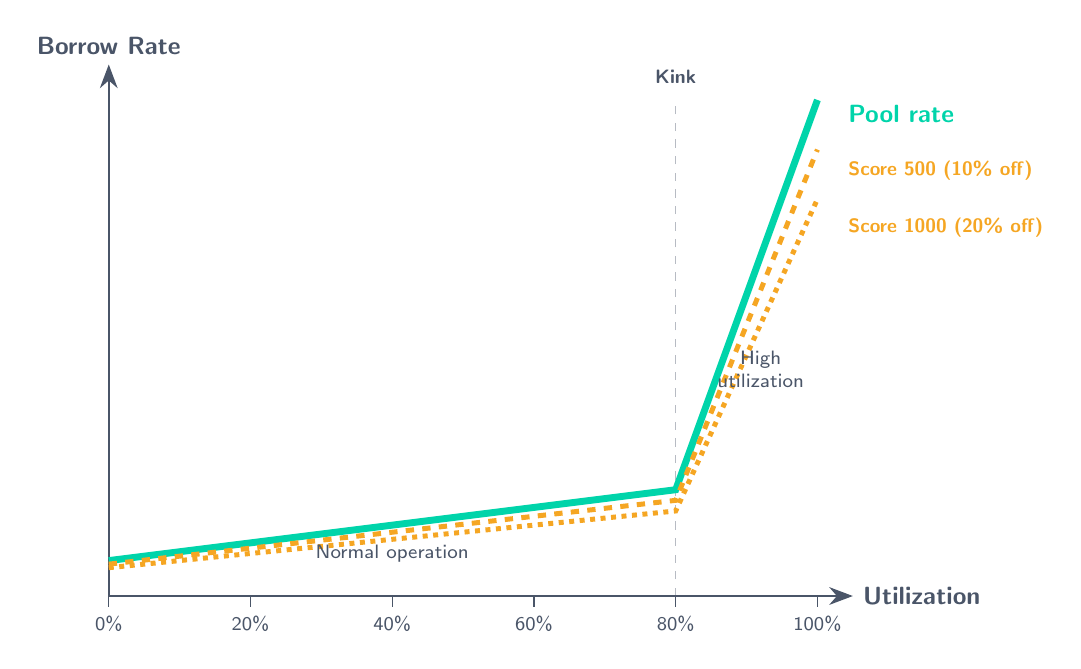
\begin{tikzpicture}[scale=0.9]
  % Axes
  \draw[-{Stealth[length=3mm]}, thick, color=TextSecondary] (0,0) -- (10.5,0) node[right, font=\small\sffamily\bfseries] {Utilization};
  \draw[-{Stealth[length=3mm]}, thick, color=TextSecondary] (0,0) -- (0,7.5) node[above, font=\small\sffamily\bfseries] {Borrow Rate};

  % Axis labels
  \foreach \x/\l in {0/0\%, 2/20\%, 4/40\%, 6/60\%, 8/80\%, 10/100\%} {
    \draw[TextSecondary] (\x,0) -- (\x,-0.15) node[below, font=\scriptsize\sffamily] {\l};
  }

  % Kink point marker
  \draw[dashed, TextSecondary, opacity=0.4] (8,0) -- (8,7);

  % Pool rate curve (base)
  \draw[PrimaryAccent, line width=2.5pt]
    (0,0.5) -- (8,1.5) -- (10,7);
  \node[PrimaryAccent, font=\small\sffamily\bfseries, anchor=west] at (10.3,6.8) {Pool rate};

  % Credit-discounted curves
  \draw[AccentGold, line width=1.8pt, dashed]
    (0,0.45) -- (8,1.35) -- (10,6.3);
  \node[AccentGold, font=\scriptsize\sffamily\bfseries, anchor=west] at (10.3,6.0) {Score 500 (10\% off)};

  \draw[AccentGold, line width=1.8pt, dotted]
    (0,0.4) -- (8,1.2) -- (10,5.6);
  \node[AccentGold, font=\scriptsize\sffamily\bfseries, anchor=west] at (10.3,5.2) {Score 1000 (20\% off)};

  % Kink label
  \node[TextSecondary, font=\scriptsize\sffamily\bfseries, anchor=south] at (8,7.1) {Kink};

  % Region labels
  \node[TextSecondary, font=\scriptsize\sffamily, text width=3cm, align=center] at (4,0.6) {Normal operation};
  \node[TextSecondary, font=\scriptsize\sffamily, text width=2.5cm, align=center] at (9.2,3.2) {High\\utilization};
\end{tikzpicture}
\caption{Interest rate curves. The base pool rate follows a two-slope kink model. Credit-scored borrowers receive a discount proportional to their score, shown for scores 500 and 1000.}
\label{fig:irm}
\end{figure}

\begin{warningbox}
The credit rate discount reduces the individual borrower's cost, not the pool rate itself. Suppliers earn the full pool rate regardless of borrower credit scores. The discount is effectively a protocol-level incentive for building credit history.
\end{warningbox}

\subsection{Liquidation}

A position is liquidatable when the borrowed value exceeds the collateral value adjusted by the borrower's effective LLTV:

\begin{equation}
\text{healthy if:}\quad \text{collateral} \times \text{price} \times \text{LLTV}_{\text{eff}} \geq \text{borrowed}
\end{equation}

Liquidators seize collateral at a discount (up to 15\% bonus), incentivizing rapid position closure. When seized collateral is insufficient to cover the debt, the residual bad debt is socialized across all suppliers in that market---contained by the isolation property of the singleton design.

The key interaction with the credit system: liquidation triggers a 100-point credit slash (Section~3.4) atomically within the same transaction. The borrower's trust tier may drop immediately, increasing their collateral requirements for any remaining positions across all markets. This creates a cascade of consequences that extends well beyond the liquidated position.

\subsection{Interest Accrual}

Interest compounds per-second using a Taylor expansion approximation:

\begin{equation}
e^{x} - 1 \approx x + \frac{x^2}{2} + \frac{x^3}{6}
\end{equation}

where $x = r \cdot \Delta t$ is the per-second rate multiplied by elapsed time. This maintains precision for the small per-second rates typical in DeFi while avoiding the computational cost of a full exponential. Accrued interest is split between suppliers and a protocol fee (capped at 25\%).

% ══════════════════════════════════════════════════════════════════════
% 5. REAL-WORLD ASSET RECEIVABLES
% ══════════════════════════════════════════════════════════════════════
\section{Real-World Asset Receivables}

Creditcoin's core mission is connecting DeFi to traditional credit infrastructure---bonds, receivables, microfinance portfolios---across emerging markets. Wikshi implements a complete receivables pipeline that takes real-world loans originated through Gluwa's lending contracts and Creditcoin's Credal-powered loan cycles and converts them into usable DeFi collateral.

\begin{figure}[H]
\centering
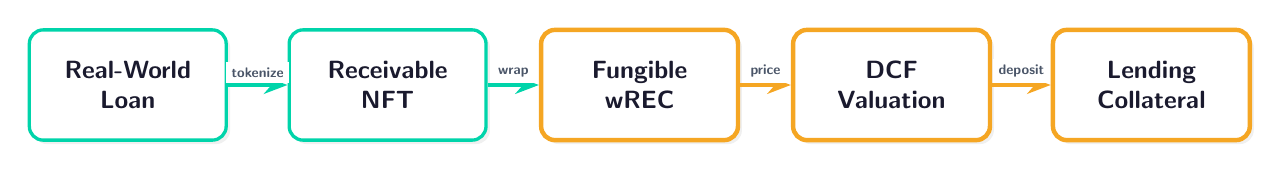
\begin{tikzpicture}[
  node distance=0.7cm,
  sbox/.style={rectangle, rounded corners=5pt, draw=PrimaryAccent, fill=white,
               text=TextPrimary, line width=1.2pt, minimum width=2.5cm, minimum height=1.4cm,
               font=\sffamily\small\bfseries, align=center,
               drop shadow={shadow xshift=0.5mm, shadow yshift=-0.5mm, opacity=0.12}},
  gold/.style={sbox, draw=AccentGold, line width=1.6pt},
  arr/.style={-{Stealth[length=3mm]}, line width=1.4pt, color=PrimaryAccent},
  garr/.style={-{Stealth[length=3mm]}, line width=1.6pt, color=AccentGold},
  lbl/.style={font=\sffamily\tiny\bfseries, color=TextSecondary, fill=white, inner sep=2pt},
]
  % Nodes
  \node[sbox] (loan) at (-6.5,0) {Real-World\\Loan};
  \node[sbox] (nft) at (-3.2,0) {Receivable\\NFT};
  \node[gold] (wrec) at (0,0) {Fungible\\wREC};
  \node[gold] (dcf) at (3.2,0) {DCF\\Valuation};
  \node[gold] (col) at (6.5,0) {Lending\\Collateral};

  % Arrows
  \draw[arr] (loan) -- node[lbl, above] {tokenize} (nft);
  \draw[arr] (nft) -- node[lbl, above] {wrap} (wrec);
  \draw[garr] (wrec) -- node[lbl, above] {price} (dcf);
  \draw[garr] (dcf) -- node[lbl, above] {deposit} (col);
\end{tikzpicture}
\caption{RWA receivable lifecycle. Real-world loans are tokenized as NFTs, wrapped into fungible ERC-20 tokens, priced via credit-adjusted DCF, and deposited as lending collateral.}
\label{fig:rwa-pipeline}
\end{figure}

\subsection{Receivable Lifecycle}

Each real-world loan receivable is tokenized as an ERC-721 NFT that embeds the full loan metadata on-chain: borrower, principal, interest rate, maturity date, repayment progress, and status. A cross-chain deduplication mechanism using source chain identifiers and loan hashes prevents the same real-world loan from being tokenized twice.

Receivables progress through a lifecycle: \emph{Active} (funded, payments expected) $\rightarrow$ \emph{Repaying} (partial payments received) $\rightarrow$ \emph{Matured} (fully repaid) or \emph{Defaulted} (missed obligations). Defaulted receivables are rejected from the wrapping pipeline---they cannot enter DeFi markets.

Individual receivable NFTs are illiquid---they represent specific loans with unique terms. A wrapping contract converts them into fungible ERC-20 tokens (wREC) denominated in a single loan currency. This makes receivables DeFi-compatible: they can be pooled, priced, and used as collateral in lending markets.

\subsection{DCF Valuation}

The receivable oracle computes the current value of each receivable using a credit-adjusted Discounted Cash Flow model:

\begin{definitionbox}{Receivable Valuation}
\[
V = R + \frac{O \times M_c \times D_t}{10^8}
\]
where:
\begin{itemize}[label={$\cdot$}]
\item $R$ = amount already repaid (fully valued, realized cash flow)
\item $O$ = outstanding balance (expected future payments)
\item $M_c$ = credit multiplier: ranges from 50\% (score~0) to 100\% (score~1000)
\item $D_t$ = time discount: ranges from 85\% (newly originated) to 100\% (at maturity)
\end{itemize}
\end{definitionbox}

The credit multiplier reflects the probability that remaining payments will be made, directly linked to the borrower's credit score. The time discount reflects the decreasing uncertainty as a loan approaches maturity---a loan with 90\% of its term elapsed is more predictable than one just funded.

\textbf{Worked example.} A \$10{,}000 microfinance receivable with \$2{,}000 already repaid, borrower score of 700, and 60\% of the loan term elapsed:
\begin{align*}
O &= \$10{,}000 - \$2{,}000 = \$8{,}000 \\
M_c &= 50\% + \frac{700}{1000} \times 50\% = 85\% \\
D_t &= 85\% + 60\% \times 15\% = 94\% \\
V &= \$2{,}000 + \$8{,}000 \times 85\% \times 94\% = \$2{,}000 + \$6{,}392 = \mathbf{\$8{,}392}
\end{align*}

This receivable, with a face value of \$10{,}000, is valued at \$8{,}392 as collateral---a 16\% haircut that reflects both the remaining credit risk and time-to-maturity discount. As the borrower makes additional payments and time progresses, the valuation converges toward the full face value.

% ══════════════════════════════════════════════════════════════════════
% 6. WORKED SCENARIOS
% ══════════════════════════════════════════════════════════════════════
\section{Worked Scenarios}

The following scenarios illustrate how Wikshi's credit system translates into concrete economic outcomes for borrowers.

\subsection{Scenario 1: Emerging Market Borrower}

\textbf{Profile.} Amara is a microfinance borrower in Lagos who has been making loan payments through Aella (a Creditcoin partner) for 18 months. She has 15 verified payments totaling \$12{,}000, with no late payments or defaults.

\textbf{Credit standing.} Through the Credal API and Creditcoin native event channels, 15 payment events have been recorded. Her credit score is 560 (initialized at 300, plus $15 \times 20 = 300$ increments for payments $\geq$\$100, minus 40 points of score decay during a 70-day gap between payments). With 15 verified payments and a score above 400, she qualifies for the Established tier.

\textbf{Borrowing comparison.} Amara wants to borrow \$5{,}000 USDT against WCTC collateral in a market with an 80\% base LLTV and 8\% pool interest rate.

\begin{table}[H]
\centering
\rowcolors{2}{PrimaryLight!30}{white}
\begin{tabularx}{\textwidth}{l X X}
\toprule
& \textbf{Standard Protocol (Aave-style)} & \textbf{Wikshi (Established tier)} \\
\midrule
Effective LLTV & 80.0\% & 85.6\% \\
Collateral required & \$6{,}250 & \$5{,}841 \\
Interest rate & 8.0\% & 7.1\% (11.2\% discount) \\
Annual interest cost & \$400 & \$355 \\
\textbf{Capital freed} & --- & \textbf{\$409} \\
\textbf{Annual savings} & --- & \textbf{\$45} \\
\bottomrule
\end{tabularx}
\caption{Scenario~1: Amara saves \$409 in posted collateral and \$45/year in interest compared to a standard overcollateralized protocol---capital she can deploy elsewhere.}
\label{tab:scenario1}
\end{table}

\subsection{Scenario 2: RWA Lender with Receivable Portfolio}

\textbf{Profile.} A microfinance institution on Creditcoin holds a portfolio of 20 active loan receivables totaling \$100{,}000 in face value. The average borrower score across these loans is 650, and the portfolio is 45\% through its average maturity.

\textbf{Collateral value.} Using the DCF valuation model:
\begin{align*}
\text{Average } M_c &= 50\% + \frac{650}{1000} \times 50\% = 82.5\% \\
\text{Average } D_t &= 85\% + 45\% \times 15\% = 91.75\% \\
V_{\text{portfolio}} &= \$35{,}000_{\text{repaid}} + \$65{,}000 \times 82.5\% \times 91.75\% = \$35{,}000 + \$49{,}208 = \mathbf{\$84{,}208}
\end{align*}

The institution wraps these receivables into wREC tokens and deposits them as collateral in a lending market. At 80\% LLTV, this enables \$67{,}366 in borrowing capacity---fresh liquidity that can fund new loans, creating a flywheel between real-world lending and DeFi capital.

\subsection{Scenario 3: Liquidation and Credit Recovery}

\textbf{Profile.} David has a credit score of 720 (Trusted tier) and an active borrow position with 87.2\% effective LLTV. A sharp price decline makes his position liquidatable.

\textbf{Consequences.} The liquidation transaction atomically:
\begin{enumerate}
\item Seizes David's collateral at a discount (up to 15\% liquidation incentive)
\item Applies a 100-point credit slash: $720 \rightarrow 620$
\item Drops David from Trusted to Established tier
\end{enumerate}

\textbf{Recovery path.} David's effective LLTV drops from 87.2\% to 86.2\% (Established tier, score 620). To return to Trusted tier, he needs to rebuild above 700 score \emph{and} maintain 20+ verified payments. At \$100+ payments, this requires at least 4 additional payments (+20 each = +80 points to reach 700), representing roughly 4--8 weeks of active borrowing.

\begin{keyinsight}
The credit recovery path creates a powerful behavioral incentive. A single liquidation erases weeks of credit building. Rational borrowers manage their positions conservatively---maintaining healthy collateral ratios even when technically allowed to borrow more---because the reputational cost of liquidation exceeds the marginal benefit of additional leverage.
\end{keyinsight}

% ══════════════════════════════════════════════════════════════════════
% 7. SECURITY & INCENTIVE ANALYSIS
% ══════════════════════════════════════════════════════════════════════
\section{Incentive Analysis and Attack Resistance}

\subsection{Participant Incentives}

\textbf{Suppliers} deposit tokens into lending markets and earn yield from borrower interest payments. Their capital is protected by overcollateralization (borrowers always post more collateral than they borrow), market isolation (a default in one market cannot affect another), and the credit tier system (higher-tier borrowers with better terms have demonstrated lower risk).

\textbf{Borrowers} are incentivized to build and maintain credit scores because the economic benefits are tangible: lower collateral requirements free capital, and interest rate discounts reduce borrowing costs. The progressive tier system creates clear milestones. A borrower approaching the Established threshold (score 400, 10 payments) has a concrete goal with a measurable reward.

\textbf{Liquidators} monitor positions for insolvency and receive a collateral bonus (up to 15\%) for closing unhealthy positions. Flash loans enable capital-efficient liquidation: a bot can borrow tokens, liquidate the position, sell the seized collateral, and repay the flash loan in a single transaction.

\subsection{Attack Resistance}

\textbf{Score farming.} An attacker might attempt to inflate their credit score by creating artificial loan payment events. Three mechanisms prevent this: (1)~a minimum \$100 payment threshold eliminates dust-transaction farming, (2)~a one-day cooldown between score updates limits the rate of accumulation, and (3)~only payments on operator-registered loans are accepted---self-transfers and circular payments are not recognized as credit events.

\textbf{Cross-chain proof forgery.} An attacker might attempt to submit forged payment proofs from a chain they control. USC's cryptographic verification makes this infeasible: the Merkle proof must correspond to a transaction actually included in the source chain's block, and the continuity proof ensures the block is part of the attested chain. Additionally, per-chain source contract allowlists prevent an attacker from deploying a malicious contract at a specific address on one chain and claiming it represents a legitimate lending contract on another.\footnote{This addresses the CREATE2 address collision attack vector, where deterministic deployment can produce identical addresses across chains.}

\textbf{Credit identity transfer.} The soulbound property of the credit token prevents a marketplace for credit scores. A borrower who has built a high score cannot sell or delegate it. A borrower who has been slashed cannot escape their reduced score by migrating to a new wallet---they would start from zero.

\textbf{Oracle manipulation.} Each market specifies its own price oracle. The credit oracle is independent of price feeds---it computes scores from verified payment events, not market data. An attacker who manipulates a price feed can create liquidation opportunities but cannot affect credit scores. Market isolation ensures that oracle manipulation in one market cannot cascade to others.

\textbf{Bad debt contagion.} The singleton architecture isolates each market. If a collateral token collapses in value and creates bad debt, the loss is socialized only among suppliers in that specific market. Suppliers in other markets are entirely unaffected. This contrasts with shared-pool designs where a single toxic collateral type can drain the entire protocol.

% ══════════════════════════════════════════════════════════════════════
% 8. COMPARISON
% ══════════════════════════════════════════════════════════════════════
\section{Comparison with Existing Protocols}

\begin{table}[H]
\centering
\footnotesize
\rowcolors{2}{PrimaryLight!30}{white}
\begin{tabularx}{\textwidth}{l C{1.6cm} C{1.6cm} C{1.5cm} C{1.5cm} C{1.5cm} C{1.5cm}}
\toprule
& \textbf{Wikshi} & \textbf{Aave V3} & \textbf{Morpho} & \textbf{3Jane} & \textbf{Goldfinch} & \textbf{Maple} \\
\midrule
Collateral & Adjusted & Fixed & Fixed & None & None & None \\
Credit data & On-chain & None & None & zkTLS & Human & Off-chain \\
Cross-chain & USC & No & No & No & No & No \\
RWA support & Yes & No & No & No & Yes & Yes \\
Architecture & Singleton & Pool & Singleton & Singleton & Pool & Pool \\
Permissionless & Yes & Gov. & Yes & No & No & No \\
Target market & Emerging & Global & Global & US credit & Emerging & Institutional \\
\bottomrule
\end{tabularx}
\caption{Protocol comparison across key design dimensions.}
\label{tab:comparison}
\end{table}

Wikshi occupies a distinct position in the DeFi lending design space. Unlike Aave V3 and Morpho Blue, it differentiates borrowers based on verified credit history. Unlike 3Jane, it maintains collateral backing for every loan---preserving the safety properties that protect suppliers. Unlike Goldfinch, it replaces human auditors with cryptographic verification, removing subjective judgment from the credit assessment process. Unlike Maple, it is permissionless and targets the broad base of emerging market borrowers rather than institutional counterparties.

The Creditcoin integration is the key architectural differentiator. No other lending protocol has access to 5M+ verified real-world loan transactions or cross-chain payment proof verification at the protocol level. This data advantage compounds over time: as more borrowers build credit history on Creditcoin, the credit oracle becomes more comprehensive, and the economic benefits of the tier system become more pronounced.

% ══════════════════════════════════════════════════════════════════════
% 9. FUTURE WORK
% ══════════════════════════════════════════════════════════════════════
\section{Future Work}

\textbf{Adaptive scoring models.} The current scoring model uses fixed increment tiers. Future versions may connect the Credal operator channel to machine learning models that incorporate richer signals---payment timing patterns, loan-to-income ratios, cross-protocol behavior, and geographic risk factors---while maintaining the same on-chain interface and trust tier structure.

\textbf{Multi-chain credit aggregation.} As Creditcoin's USC infrastructure supports additional source chains, the credit oracle automatically gains access to a wider set of verifiable payment history. A borrower's Ethereum lending history, Polygon microfinance payments, and Creditcoin native transactions can all contribute to a single composite credit profile. No contract upgrade is needed---new chains are registered through the existing administrative interface.

\textbf{Institutional receivable markets.} The RWA pipeline currently targets microfinance receivables. The same architecture supports larger asset classes: trade finance receivables, invoice factoring, equipment leasing, and structured credit products. As Creditcoin's real-world asset infrastructure matures, Wikshi can serve as the DeFi pricing and collateralization layer for a broad range of credit instruments.

\textbf{Governance and decentralization.} Protocol parameter management---market curation, fee structures, oracle operator registration---will transition to a governance token and DAO structure, enabling the community to direct protocol evolution while maintaining the security guarantees of the core smart contracts.

% ══════════════════════════════════════════════════════════════════════
% REFERENCES
% ══════════════════════════════════════════════════════════════════════

\renewcommand{\refname}{}
\section*{References}
\addcontentsline{toc}{section}{References}
\vspace{-2em}

\begin{thebibliography}{99}

\bibitem{morpho}
Morpho Labs. ``Morpho Blue: Permissionless Lending Protocol.'' Technical Documentation. \url{https://docs.morpho.org/}

\bibitem{creditcoin}
Creditcoin Foundation. ``Universal Smart Contract (USC) Documentation.'' \url{https://docs.creditcoin.org/}

\bibitem{goldfinch}
Goldfinch Finance. ``Goldfinch: Trust Through Consensus.'' Whitepaper v1.1, July 2021.

\bibitem{threejane}
3Jane Protocol. ``3Jane: Credit-Based Money Market Protocol.'' Whitepaper v1.1, October 2025.

\bibitem{binance-rwa}
Binance Research. ``Real World Assets: The Bridge Between TradFi and DeFi.'' March 2023.

\bibitem{aave}
Aave. ``Aave V3 Technical Paper.'' \url{https://docs.aave.com/}

\bibitem{maple}
Maple Finance. ``Institutional Lending Protocol.'' \url{https://maple.finance/}

\bibitem{eip4626}
EIP-4626. ``Tokenized Vault Standard.'' Ethereum Improvement Proposals.

\bibitem{eip5192}
EIP-5192. ``Minimal Soulbound NFTs.'' Ethereum Improvement Proposals.

\bibitem{eip712}
EIP-712. ``Typed Structured Data Hashing and Signing.'' Ethereum Improvement Proposals.

\end{thebibliography}

\vfill

\begin{center}
\color{TextSecondary}\small\sffamily
Built for the BUIDL CTC Hackathon $\cdot$ March 2026
\end{center}

\end{document}
